\section{Additional Evaluation}\label{app:evaluation}

\begin{figure*}
    \begin{subfigure}[b]{0.25\linewidth}
        \centering
        %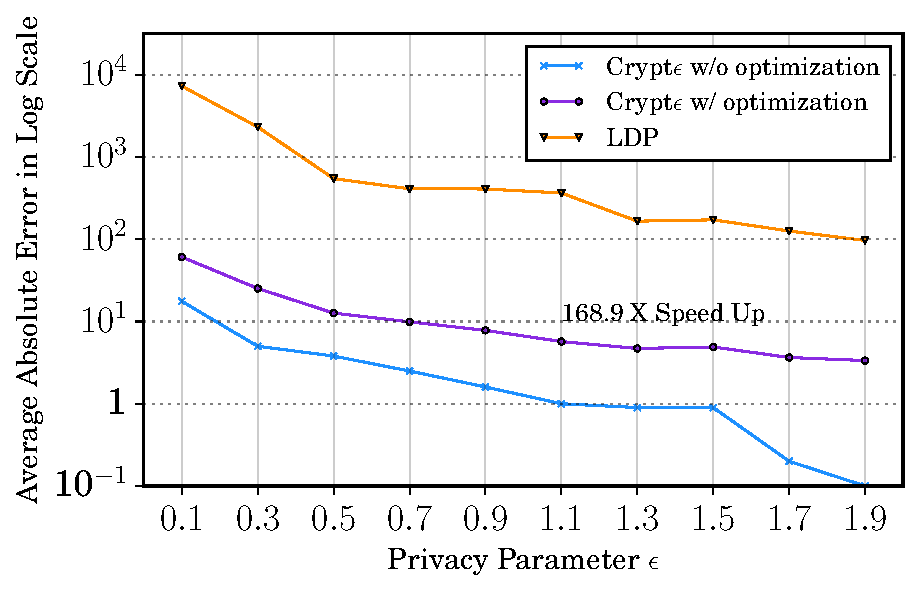
\includegraphics[width=5cm,height=3.1cm]{t1.pdf}
         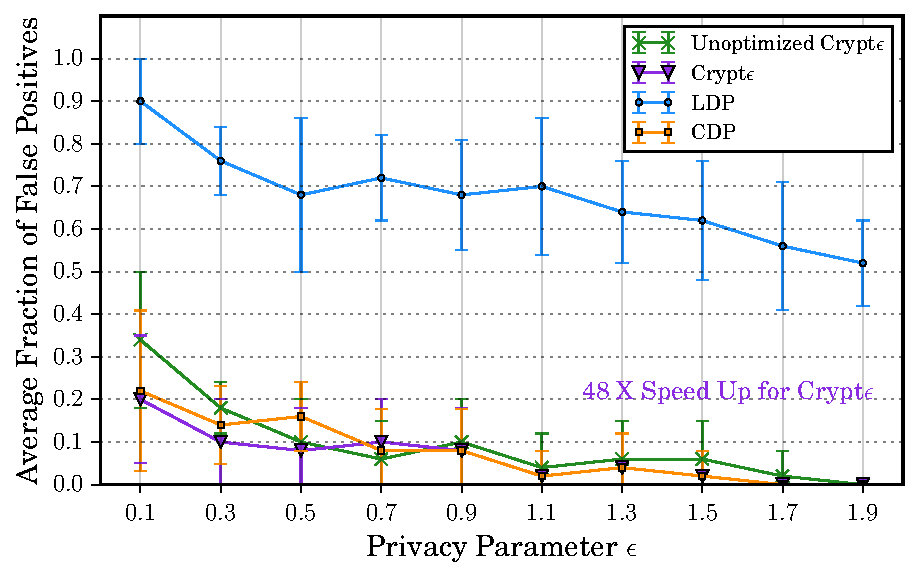
\includegraphics[width=1\linewidth]{2_final.pdf}
        \caption{ Program 2}
        \label{fig:P2}
    \end{subfigure}
    \begin{subfigure}[b]{0.25\linewidth}
    \centering 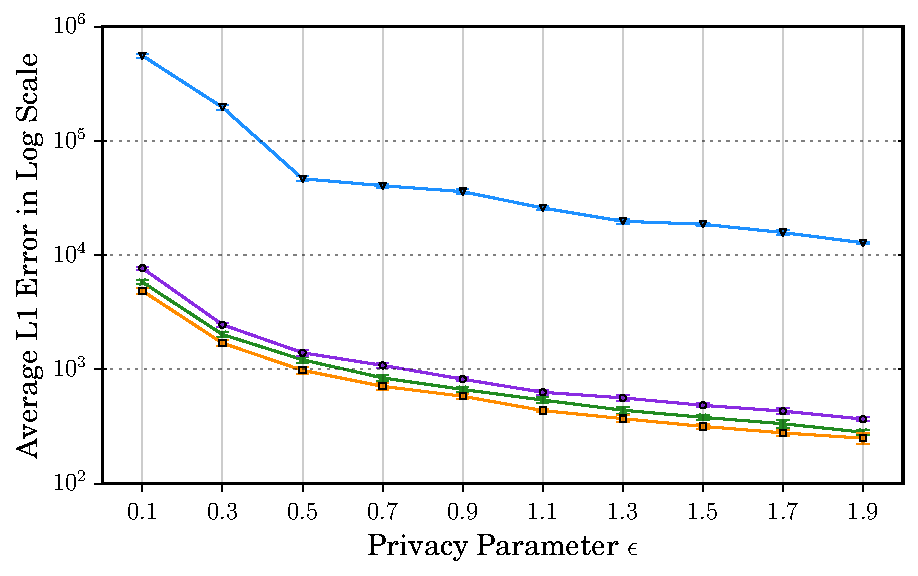
\includegraphics[width=1\linewidth]{4_final.pdf}
        \caption{Program 4}
        \label{fig:P4}\end{subfigure}
    \begin{subfigure}[b]{0.25\linewidth}
    \centering    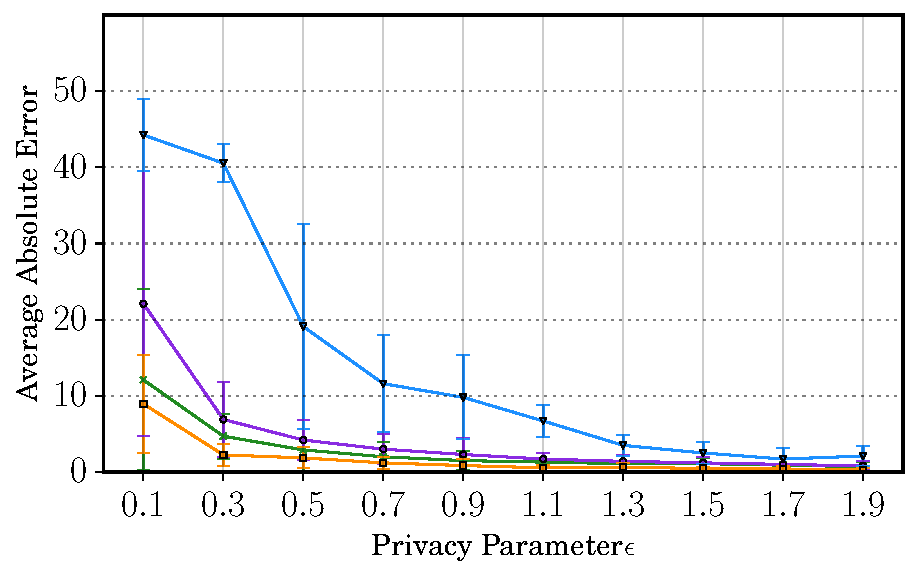
\includegraphics[width=1\linewidth]{6_finals.pdf}
        \caption{Program 6}
        \label{fig:P6}\end{subfigure}
   \caption{Accuracy Analysis of Crypt$\epsilon$ Programs Cntd.}
   \label{accuracy-appendix}
\end{figure*}

We present additional accuracy study for \system programs P2, P4, and P6 from Table~\ref{tab:programexamples}. Figure~\ref{accuracy-appendix} shows the empirical accuracy of these three programs (both optimized and unoptimized) and that of the corresponding state-of-the-art \textsf{LDP} \cite{LDP1} and \textsf{CDP} \cite{Dork} implementations  with varying privacy parameter $\epsilon \in \{0.1,...,0.9\}$. We observe similar results for P2, P4, and P6 as that of the other programs (P1, P3, P5, P7 in Figure~\ref{accuracy}). The error values of \system  and unoptimized \system  are very close to that of \textsf{CDP} and are much smaller than that of \textsf{LDP}.
